\documentclass[aspectratio=169]{beamer}

\usetheme{Madrid}
\usecolortheme{default}

\usepackage[utf8]{inputenc}
\usepackage{booktabs}
\usepackage{graphicx}
\usepackage{amsmath}
\usepackage{tikz}
\usetikzlibrary{positioning, arrows.meta}

\title[OR Capacity Planning]{Multi-Objective Operating Room Capacity Planning\\ and Utilization Optimization Using Surgical Workflow Analytics}
\author{}
\institute{}
\date{}

\begin{document}

% ---------- Slide 1: Title ----------
\begin{frame}
    \titlepage
    \vspace{-1.2cm}
    \begin{center}
        \textbf{Student Details:}\\[4pt]
        \begin{tabular}{ll}
        1. Student Name 1 & -- Roll No. 1 \\
        2. Student Name 2 & -- Roll No. 2 \\
        3. Student Name 3 & -- Roll No. 3 \\
        4. Student Name 4 & -- Roll No. 4 \\
        \end{tabular}\\[6pt]
        \textbf{Team Number:} XX
    \end{center}
\end{frame}

% ---------- Slide 2: Problem Statement ----------
\begin{frame}{Problem Statement}
    \begin{itemize}
        \item A hospital operates \textbf{8 Operating Room (OR) suites}
        shared across \textbf{10 surgical specialties} (Orthopedics,
        Podiatry, ENT, OBGYN, and others).
        \item Every week, hospital administration must decide \textbf{how
        many hours of OR block-time to give to each specialty}.
        \item Giving a specialty too few hours wastes expensive OR capacity
        that could have been used elsewhere.
        \item Giving one specialty too many hours starves the others and
        pushes cases into costly overtime.
        \item Using one quarter of actual surgical records (bookings,
        actual start/end times, OR suite used), the hospital wants to find
        the weekly OR-hour allocation across the 10 specialties that
        performs the \textbf{maximum number of surgical cases}.
        \item This allocation must not exceed the hospital's total OR
        capacity, and must not stray far from what each specialty has
        historically needed.
    \end{itemize}
    \vspace{6pt}
    \textbf{Key Challenge:} Maximizing throughput alone can push overtime and
    idle time to unsafe levels -- so the model is later extended to also
    control overtime, making it a \textbf{multi-objective} decision.
\end{frame}

% ---------- Slide 3: Dataset Description ----------
\begin{frame}{Dataset Description}
    \begin{center}
    \small
    \begin{tabular}{ll}
        \toprule
        \textbf{Attribute} & \textbf{Meaning} \\
        \midrule
        Date & Date of the surgery \\
        OR Suite & Operating room (1--8) where the surgery took place \\
        Service & Surgical specialty (e.g. Orthopedics, ENT) \\
        CPT Code / Description & Standard procedure code and description \\
        Booked Time (min) & Time originally scheduled for the surgery \\
        OR Schedule & Scheduled start time \\
        Wheels In / Wheels Out & Patient arrival in / departure from OR \\
        Start Time / End Time & Actual surgery start and end time \\
        \bottomrule
    \end{tabular}
    \end{center}
    \vspace{8pt}
    \textbf{Source:} Public OR Utilization dataset, Q1 2022 (2{,}172 surgical
    records) -- Kaggle: \textit{Optimizing Operating Room Utilization}\\
    \url{https://www.kaggle.com/datasets/thedevastator/optimizing-operating-room-utilization}
\end{frame}

% ---------- Slide 4: Statistical Analysis ----------
\begin{frame}{Statistical Analysis}
    From the raw timestamps, we compute:
    \[
        \text{Actual Duration} = \text{End Time} - \text{Start Time}
        \qquad
        \text{Overtime} = \max(0,\ \text{Actual Duration} - \text{Booked Time})
    \]
    \[
        \text{Utilization \%} = \frac{\text{Total Actual Duration (suite, day)}}
        {\text{Last Wheels Out} - \text{First Wheels In (suite, day)}}
    \]
    \vspace{4pt}
    These are summarized into an \textbf{on-demand statistics dashboard}:
    \begin{itemize}
        \item Enter an \textbf{OR Suite number} $\rightarrow$ see its average
        utilization \%, total hours used, and number of active days.
        \item Enter a \textbf{Service name} $\rightarrow$ see its case count,
        average actual duration, average overtime, and average booked time.
    \end{itemize}
    Average OR utilization across all suites in Q1 2022 was found to be
    \textbf{$\sim$46\%} -- indicating significant unused capacity.
\end{frame}

% ---------- Slide 5: Proposed Solution ----------
\begin{frame}{Proposed Solution}
    \begin{enumerate}
        \item Clean the raw dataset and compute per-case duration, overtime,
        turnover, and per-suite-per-day utilization.
        \item Build an on-demand statistics dashboard for the user to explore
        the data by OR Suite or by Service.
        \item Formulate the weekly OR-hour allocation decision as a
        \textbf{Linear Programming (LP)} problem that maximizes surgical
        throughput.
        \item Solve the LP using \textbf{Excel Solver} and generate a
        \textbf{Sensitivity Report} to see which constraints limit the hospital.
        \item Extend the model to \textbf{Goal Programming}, so the hospital
        can balance throughput \emph{and} overtime instead of only maximizing cases.
    \end{enumerate}
\end{frame}

% ---------- Slide 6: LP Formulation ----------
\begin{frame}{Linear Programming Model}
    \footnotesize
    \textbf{Decision variable:} $X_s$ = OR-hours allocated to specialty $s$ per week

    \begin{center}
    \begin{tabular}{lcccc}
        \toprule
        \textbf{Specialty} & \textbf{Avg. Duration (min)} & \textbf{Min. Hours} & \textbf{Max. Hours} \\
        \midrule
        ENT            & 33.9 & 6.9  & 10.3 \\
        Orthopedics    & 58.2 & 19.2 & 28.7 \\
        Podiatry       & 56.3 & 14.2 & 21.3 \\
        Plastic        & 69.0 & 14.7 & 22.0 \\
        \multicolumn{4}{c}{\textit{(and 6 more specialties, same format)}} \\
        \bottomrule
    \end{tabular}
    \end{center}

    \textbf{Objective:} Maximize total weekly cases performed
    \[
        \text{Maximize } Z = \sum_{s=1}^{10} \frac{60\, X_s}{D_s}
    \]
    \textbf{Subject to:}
    \[
        \sum_{s=1}^{10} X_s \leq 320 \ \text{(total weekly OR capacity)}, \qquad
        \text{Min. Hours}_s \leq X_s \leq \text{Max. Hours}_s, \qquad X_s \geq 0
    \]
    \textbf{Result (Excel Solver, Simplex LP):} $Z^{*} = 200.49$ cases/week,
    using only 152 of 320 available hours.
\end{frame}

% ---------- Slide 7: Goal Programming ----------
\begin{frame}{Goal Programming Model}
    The LP alone maximizes cases but completely ignores overtime. In practice
    the hospital cares about \textbf{both}, so two goals are set instead of
    one objective:

    \vspace{6pt}
    \textbf{Goal 1 -- Throughput:} total weekly cases should be close to the
    LP optimum (200 cases)
    \[
        \sum_{s} \frac{60\, X_s}{D_s} + d_1^- - d_1^+ = 200
    \]
    \textbf{Goal 2 -- Overtime:} total weekly overtime should stay low
    \[
        \sum_{s} \text{Overtime}_s + d_2^- - d_2^+ = \text{Target Overtime}
    \]
    \textbf{Objective:} Minimize the (weighted) amount by which each goal is missed
    \[
        \text{Minimize } W_1\, d_1^- + W_2\, d_2^+
    \]
    This is what makes the project \textbf{multi-objective}: instead of one
    number to optimize, the hospital balances two competing priorities.
\end{frame}

% ---------- Slide 8: Methodology ----------
\begin{frame}{Methodology}
    \centering
    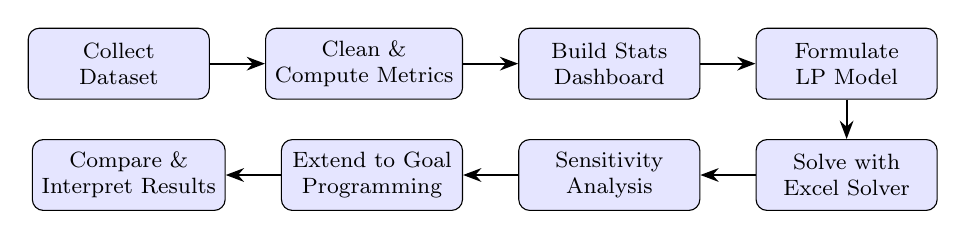
\begin{tikzpicture}[
        node distance=0.5cm and 0.7cm,
        box/.style={rectangle, rounded corners, draw, fill=blue!10, minimum width=2.3cm, minimum height=0.9cm, align=center, font=\footnotesize},
        arr/.style={-Stealth, thick}
    ]
        \node[box] (a) {Collect\\Dataset};
        \node[box, right=of a] (b) {Clean \&\\Compute Metrics};
        \node[box, right=of b] (c) {Build Stats\\Dashboard};
        \node[box, right=of c] (d) {Formulate\\LP Model};
        \node[box, below=of d] (e) {Solve with\\Excel Solver};
        \node[box, left=of e] (f) {Sensitivity\\Analysis};
        \node[box, left=of f] (g) {Extend to Goal\\Programming};
        \node[box, left=of g] (h) {Compare \&\\Interpret Results};

        \draw[arr] (a) -- (b);
        \draw[arr] (b) -- (c);
        \draw[arr] (c) -- (d);
        \draw[arr] (d) -- (e);
        \draw[arr] (e) -- (f);
        \draw[arr] (f) -- (g);
        \draw[arr] (g) -- (h);
    \end{tikzpicture}
\end{frame}

% ---------- Slide 9: Techniques & Tools ----------
\begin{frame}{Techniques \& Tools}
    \begin{center}
    \begin{tabular}{ll}
        \toprule
        \textbf{Tool} & \textbf{Role} \\
        \midrule
        Microsoft Excel & Data platform and user interface \\
        Power Query & Importing and cleaning raw data \\
        Excel Formulas (SUMIFS, MINIFS, MAXIFS) & Computing statistics on demand \\
        Excel Solver (Simplex LP) & Solving LP and Goal Programming models \\
        Sensitivity / Answer / Limits Reports & Interpreting the optimal solution \\
        \bottomrule
    \end{tabular}
    \end{center}
\end{frame}

% ---------- Slide 10: Results / Comparative ----------
\begin{frame}{Results}
    \begin{center}
    \begin{tabular}{lcc}
        \toprule
        \textbf{Metric} & \textbf{Before (Current Practice)} & \textbf{After (LP-Optimized)} \\
        \midrule
        Avg. OR Utilization & $\sim$46\% & Capacity-aware allocation \\
        Weekly Surgical Cases & Historical average & \textbf{200.49 (maximum feasible)} \\
        OR Capacity Used & Unmeasured & 152 of 320 hours (48\%) \\
        Binding Constraint & -- & Specialty demand caps, \emph{not} capacity \\
        \bottomrule
    \end{tabular}
    \end{center}
    \vspace{10pt}
    \textbf{Key Insight:} The hospital is not capacity-constrained -- OR
    capacity has significant headroom. The real limitation is how each
    specialty's demand bounds were set, which the Sensitivity Report exposes.
\end{frame}

% ---------- Slide 11: Significance ----------
\begin{frame}{Significance}
    \begin{enumerate}
        \item \textbf{Capacity Insight} -- Reveals whether OR capacity or
        specialty demand limits is the actual bottleneck.
        \item \textbf{Overtime Awareness} -- Goal Programming keeps overtime
        in check instead of chasing throughput alone.
        \item \textbf{Data-Driven Scheduling} -- Allocation is grounded in
        one quarter of real surgical records, not guesswork.
        \item \textbf{Multi-Objective Decision Making} -- Administrators can
        weigh throughput against overtime instead of being locked into one goal.
    \end{enumerate}
    \vspace{10pt}
    \textbf{Operations Research Application:} Linear Programming, Goal
    Programming, and Sensitivity Analysis applied to real hospital operating
    room capacity planning.
\end{frame}

\end{document}
